\begin{abstract}
Visual examples provide a flexible way to specify segmentation targets without task-specific retraining. In-context segmentation (ICS) uses an annotated reference to predict a target mask in a query image. This study compares INSID3 and CG-ICS on COCO-$20^i$ and LVIS-$92^i$ through accuracy, reference sensitivity, and inference cost. CG-ICS achieves mean-fold class-pooled IoU of 72.17\% and 47.44\%, versus 57.65\% and 40.77\% for INSID3. On inputs matched by runner GPU model, its mean inference latency is 7.37--10.63 times higher, with an additional language-model GPU. Ablations identify substantial gains from INSID3's feature processing and CG-ICS's combination of semantic concepts and visual prompts. Further search adds 0.22 equal-query IoU points on COCO and 2.30 on LVIS, with smaller marginal gains when visual prompts are present. These findings motivate Agreement-Gated Search (AGS), which uses text--visual mask agreement to allocate concept search. A cost--accuracy decomposition identifies the computation savings and prediction changes that determine its value. Code is available at \url{https://github.com/AvianHan/CE6190-Visual-Understanding}.
\end{abstract}

\section{Introduction}
Visual examples allow users to specify segmentation targets beyond a fixed vocabulary, avoiding the need to annotate every new image. In-context segmentation (ICS) implements this interface using a reference image and its binary mask to identify the corresponding target in a query image. The transfer can fail when appearance changes, the reference captures only part of the target, or similar objects compete in the query. Effective ICS must therefore combine accurate target identification, consistency across references, and affordable inference.

Two recent training-free systems illustrate different ways of using the reference. INSID3 constructs a mask from frozen DINOv3 features through debiasing, clustering, and similarity aggregation~\cite{insid3,dinov3}. CG-ICS generates and searches language concepts from the reference, then combines the selected concept with visual prompts in SAM~3~\cite{cgics,sam3}. The comparison connects two forms of visual understanding: dense correspondence that transfers spatial evidence, and semantic interpretation that converts an example into a concept.

Their different designs raise questions beyond average segmentation accuracy. How much does performance change with the reference, which processing stages account for the gains, and when is additional search worth its cost? Answering these questions requires matched system comparisons together with component interventions and measured computation. In particular, input-dependent search becomes attractive if the benefits of further reasoning vary across queries.

This work examines these questions on COCO-$20^i$ and LVIS-$92^i$ using common reference/query inputs. CG-ICS achieves higher accuracy, while INSID3 provides a faster inference path; component analysis shows that visual prompts reduce the marginal return from concept search. This observation motivates the hypothesis that agreement between text-only and visual-only masks can identify inputs with limited need for further search. Agreement-Gated Search (AGS) turns this hypothesis into a decision rule, accompanied by a cost--accuracy analysis and controlled evaluation design. The contributions are threefold:
\begin{enumerate}[label=(\arabic*),leftmargin=1.7em,itemsep=4pt]
\item \textbf{Paired system evaluation.} A comparison of accuracy, reference sensitivity, and computational cost on common inputs.
\item \textbf{Component analysis.} Controlled ablations of feature processing, semantic search, visual prompting, and backbone choice.
\item \textbf{Agreement-Gated Search.} A proposed input-dependent search rule with an explicit cost--accuracy formulation and evaluation controls.
\end{enumerate}

\begin{figure*}[t]
    \centering
    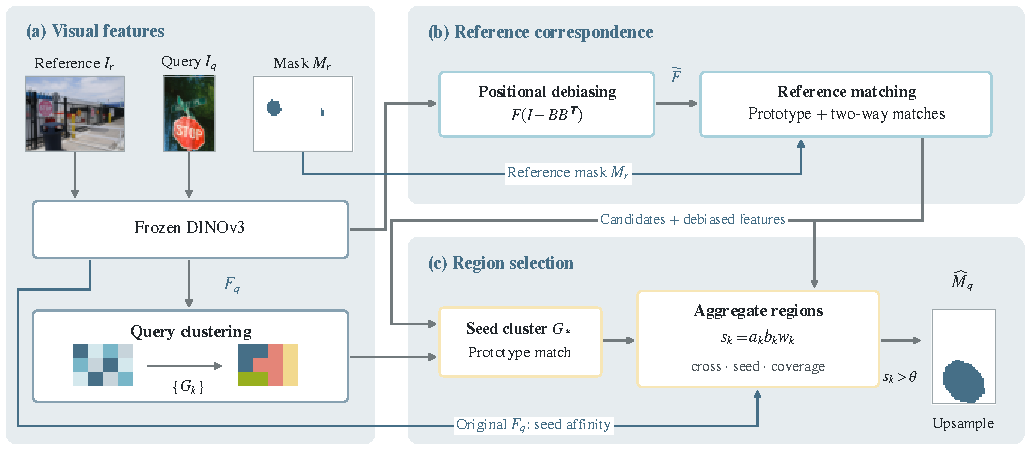
\includegraphics[width=\linewidth]{figures/insid3_pipeline.pdf}
    \caption{\textbf{INSID3.} Original features support region grouping; debiased features guide reference matching and seed selection. Selected clusters form the query mask.}
    \label{fig:insid3}
\end{figure*}
